\documentclass{article}
\usepackage[utf8]{inputenc}
\usepackage{graphicx}
\usepackage{color}
\title{sea view}


\begin{document}
\begin{center}
    
\includegraphics{aiublogo.jpg}
\end{center}
\begin{code}
\textbf{American International University of Bangladesh}

\end{code}
\begin{code}
\color{red}{Computer Graphics - Project Documentation }
\end{code} \\
\\
\begin{center}
\begin{tabular}{c|c}
    \hline
    Course name  & Computer Graphics \\
    \hline
    Course Teacher & Md Masum Billah \\
    \hline
    Section & B
\end{tabular}
\end{center}


\begin{center}
  \begin{code}
\textbf{Group Members:}

\end{code}  
\end{center}
\begin{center}
\begin{tabular}{c|c}
    \hline
   Name  & Id \\
    \hline
    Hrichik Paul Ankan & 20-41940-1 \\
    \hline
    Kakon, Khairul Islam & 20-42438-1 \\
    \hline
    Md. Rahamatullah & 19-40946-2 \\
    \hline
    faysal & 2fdfsdf324 \\
    \hline
\end{tabular}
\end{center}\
\\

\begin{center}
  \begin{code}
\textbf{Table of Content}

\end{code}  
\end{center}
\begin{center}
\begin{tabular}{c|c}
    \hline
   \textbf{Content List}  & \textbf{Page No} \\
    \hline
    Introduction & 03 \\
    \hline
    Proposal & 03 \\
    \hline
    Schematic Diagram & 04\\
    \hline
    List of Objects & 04-06 \\
    \hline
    Functions to Represent the Objects & 06-08 \\
    \hline
    Interactive Functions & 09 \\
    \hline
    Task Assignment and Codes of Functions & 10-11 \\
    \hline
    output & 12-14 \\
    \hline
    Conclusion & 14 \\
    
    
\end{tabular}
\\
\end{center}

\begin{center}
    \textbf{Introduction}
    \\
    The concept will showcase a seashore setting with a simplistic appearance. We created a scenario with three views: day, night, and evening. When the button is pressed, the rain will appear in each perspective. Each different scene will have a sound effect. When taken as a whole, it would produce an attractive sea beach scene. Our application renders the objects quickly and precisely. as well as a setting meant to resemble a beach.
\end{center}
\\
\begin{center}
    \textbf{Proposal}
    \\
    A scenario-related project. A "cox's Bazar view" real-world scenario will be shown. Mountain, seat, umbrella, sun, moon, stars at night, trees, sand, balloon, tower, and mill will all be present. There will be some sort of keyboard connection established. The scenario will start with a keyboard and a rain view.
\end{center}

\begin{center}
    \textbf{Schematic Diagram}
  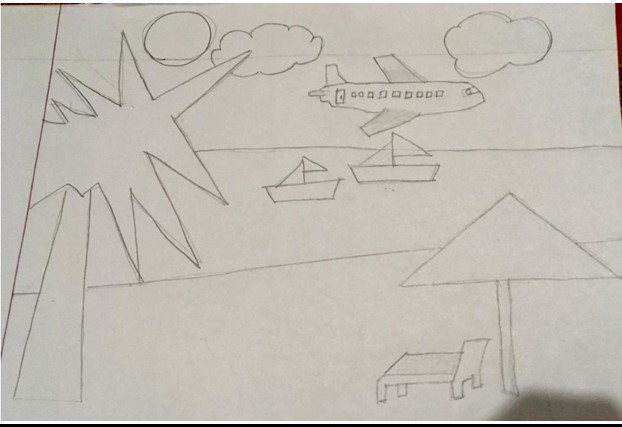
\includegraphics[]{schematic.jpg}\\
  \\
\end{center}
\\
\begin{center}
    \\
\end{center}
\begin{center}
    \\
\end{center}
\\
 \begin{align}
    \begin{center}
        \textbf{List Of Objects}
    \end{center} \\
    
    \textbf{1)}	Boat1\\
     \textbf{2)}	Boat2\\
\textbf{3)}	Rain\\
\textbf{4)}	Day Sun\\
\textbf{5)}	Evening Sun\\
\textbf{6)}	 Moon\\
\textbf{7)}	Cloud1\\
\textbf{8)}	Cloud2\\
\textbf{9) } Bird1\\
\textbf{10)}	Bird2\\
\textbf{11)}	Tree\\
\textbf{12)}	Umbrella\\
\textbf{13)}	Seat\\
\textbf{14)}	Plane\\
\textbf{15)}	Balloon\\
\textbf{16)}	Day sky\\
\textbf{17)}	Evening sky\\
\textbf{18)}	Night sky\\
\textbf{19)}	Stars\\
\textbf{20)}	Day sea\\
\textbf{21)}	Evening sea\\
\textbf{22)}	Night sea\\
\textbf{23)}	Rainy sea\\
\textbf{24)}	Rain Sand\\
\textbf{25)}	Day Sand\\
\textbf{26)}	Evening sand\\
\textbf{27)}	Night sand\\

 \end{align}
\\
\begin{center}
    \\
\end{center}
\begin{center}
    \\
\end{center}\\
\begin{center}
    \\
\end{center}
\begin{center}
    \\
\end{center}\\
\begin{center}
    \\
\end{center}
\begin{center}
    \\
\end{center}
\begin{center}
    \\
\end{center}
\begin{center}
    \\
\end{center}
\begin{center}
    \\
\end{center}
\begin{center}
  \begin{code}
  
\textbf{Functions to Represent The objects}

\end{code}  
\end{center}
\begin{center}
\begin{tabular}{c|c}
    \hline
   \textbf{Object}  & \textbf{Function} \\
    \hline
    boat 1 & Void boat1() \\
    \hline
    boat 2 & Void boat2() \\
    \hline
    Plane & Void Plane()\\
    \hline
     Rain & Void rain() \\
    \hline
    Sun & void sun() \\
    \hline
    Moon & Void Mood()\\
    \hline
    Cloud1 & Void Cloud1() \\
    \hline
    Cloud2 & Void Cloud2() \\
    \hline
    Bird1 & Void Bird1() \\
    \hline
    Bird2 & Void Bird2() \\
    \hline
    Tree & Void Tree() \\
    \hline
    Umbrella & Void Umbrella() \\
    \hline
    Seat & Void Seat() \\
    \hline
    Hot Ballon & Void Hot Ballon() \\
    \hline
    Day Sky & Void Day Sky() \\
    \hline
    Evening sky & Void Evening Sky() \\
    \hline
     Rainy Sky & Void Rainy Sky() \\
    \hline
     Stars & Void Stars() \\
    \hline
     Night Sky & Void Night Sky() \\
    \hline
    Day Sea & Void  Day Sea() \\
    \hline
     Evening Sea & Void Evening Sea() \\
    \hline
     Night Sea & Void Night Sea() \\
    \hline
     Rainy Sea & Void Rainy Sea() \\
    \hline
    Rainy sand & Void Rainy sand() \\
    \hline
    Day Sand & Void Day Sand() \\
    \hline
    Night Sand & Void Night Sand() \\
    
    
    
    
\end{tabular}
\\
    \\
\end{center}
\begin{center}
  \begin{code}
\textbf{Interactive Functions}

\end{code}  
\end{center}
\begin{center}
\begin{tabular}{c|c}
    \hline
   \textbf{Interactive Functions}  & \textbf{Interaction} \\
    \hline
    Update_sun & sun_update \\
    \hline
    update_boat1	& boat1_update,boat1_ move\\
    \hline
    update_boat2	& Boat2_update,boat1_ move\\
    \hline
    Update_plane	& Plane_move , Plane_update\\
    \hline
     update_moon	&  moon_move, moon_update\\
     \hline
    update_cloud1 &	Cloud1_update\\
    \hline
    update_cloud2	& Cloud2_update\\
    \hline
    update_hotballoon	 & hotballoon_update\\
    \hline
    update_bird1	& Bird1_update,bird1_move\\
    \hline
    update_bird2	& Bird2_update,bird2_move\\
    \hline
    update_rain	& rain_move, rain_update\\
    
    
\end{tabular}
\\
\end{center}
\begin{center}
    \\
\end{center}
\begin{center}
    \\
\end{center}

\begin{center}
  \begin{code}
\textbf{Task Assignment and Codes of Functions}

\end{code}  
\end{center}
\textbf{Contribution Table:(per Percent) }
\begin{center}
\begin{tabular}{c|c|c|c|c}
    \hline
   \textbf{Member-1 }  & \textbf{Member-2 } & \textbf{Member-3}& \textbf{Member-4}& \textbf{Total}\\
    \hline
    \begin{center}
        \color{blue}{25}
    \end{center}
     & \begin{center}
        \color{blue}{25}
    \end{center}
     & \begin{center}
        \color{blue}{25}
    \end{center}
     & \begin{center}
        \color{blue}{25}
    \end{center}
     & \begin{center}
        \color{blue}{100}
    \end{center}
    
    
    
    
\end{tabular}
\\
\end{center}

\begin{center}
\begin{tabular}{c|c}
    \hline
   \textbf{\color{blue}{Name/ID} }  & \textbf{\color{blue}{Contribution On project} }\\
    \hline
    Hrichik Paul &  \textbf{1} Night sea\\ 
               20-41940-1    &  \textbf{ 2.}	Evening sea\\
                   &   \textbf{3.}	Rainy sea\\
                    & \textbf{ 4.}	Cloud1\\
                    & \textbf{ 5.}	Big tree\\
                   &  \textbf{ 6.}	Umbrella\\
                   &  \textbf{ 7.}	Stand\\
                   &   \textbf{8.}	Boat1\\
                  &   \textbf{ 9.}	Boat2\\
                  \hline \\
    kakon, Khairul Islam & \textbf{1.}	Ship1\\
         20-42438-1        &\textbf{2.}	Rain\\
                 &\textbf{3.}	Bird\\
                 &\textbf{4.}	Evening sky\\
                 &\textbf{5.}	Night sky\\
                 &\textbf{6.}	Sea texture\\
                 &\textbf{7.}	Sea wave\\
                 &\textbf{8.}	Day sand texture\\
                 &\textbf{9.}	Event Handler\\
                 \hline \\
    Md. Rahamatullah & \textbf{1.}	Evening sea \\
           19-40946-2    &\textbf{2.}	Night sea\\
               &\textbf{3.}	Day mountain\\
               &\textbf{4.}	Evening mountain\\
               &\textbf{5.}	Night mountain\\
               &\textbf{6.}	Night sand\\
               &\textbf{7.}	Evening sand\\
               &\textbf{8.}Night sand texture\\
                \hline \\
    Foysal & \textbf{1.}	Ship2\\
             & \textbf{2.}	Seat\\
             & \textbf{3.}	Umbrella\\
             & \textbf{4.}	Stars\\
             & \textbf{5.}	Tree\\
             & \textbf{6.}	Tower\\
             & \textbf{7.}	Day sand\\


                 


    
    
    
    
    
\end{tabular}
\\
\end{center}

\begin{center}
    \textbf{Output}
   \begin{figure}
       \centering
       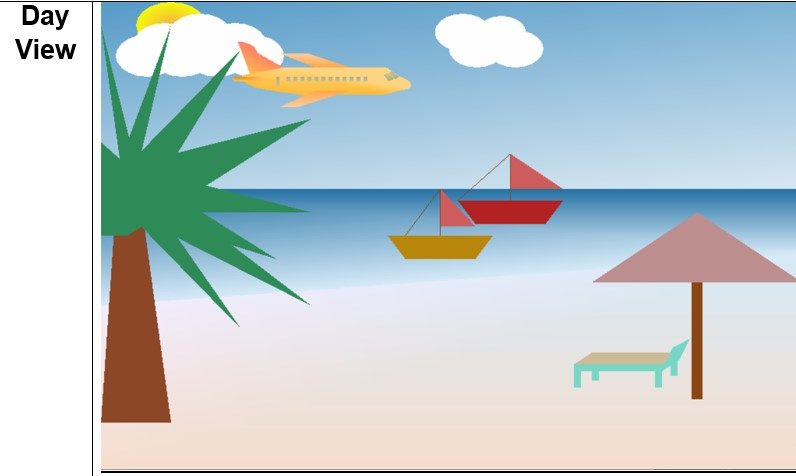
\includegraphics[width=5in]{Day View.jpg}\\
    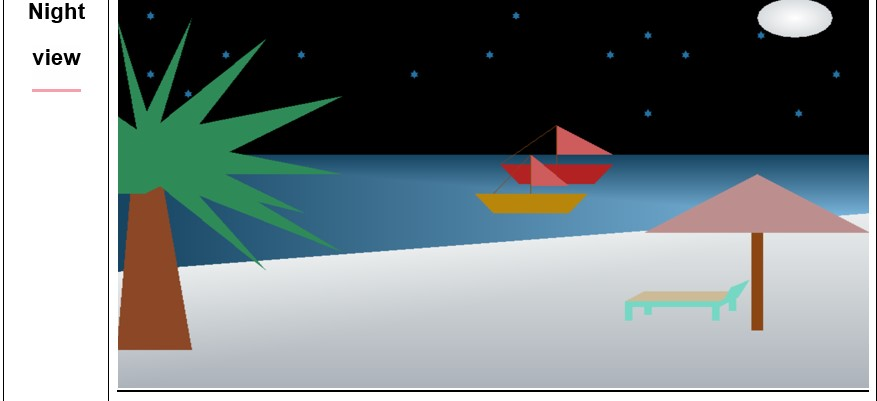
\includegraphics[width=5in]{Night View.jpg}\\
    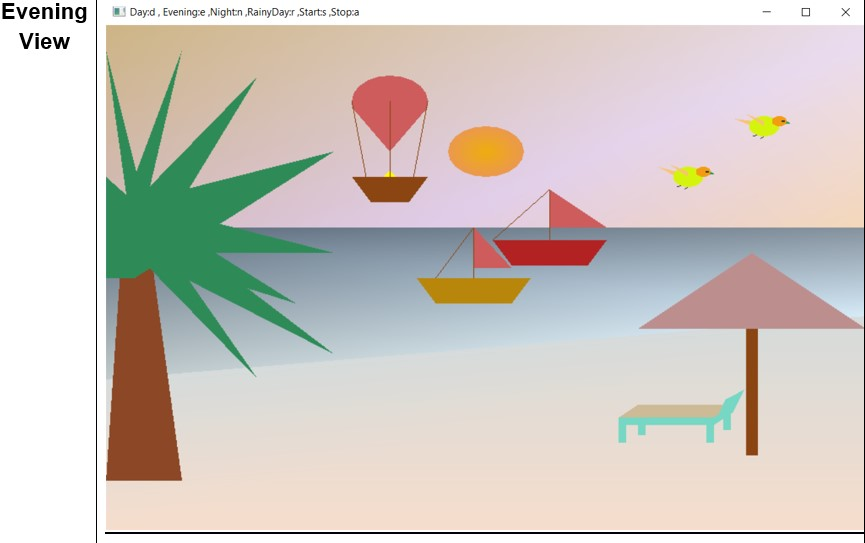
\includegraphics[width=5in]{Evening view.jpg}\\
    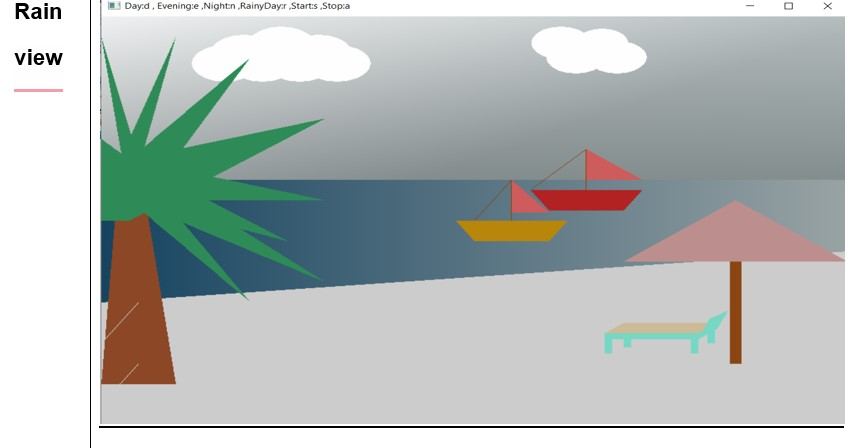
\includegraphics[width=5in]{rain view.jpg}\\
      
   \end{figure} 
\end{center}



\end{document}
